\documentclass[10pt]{beamer}

\usetheme[progressbar=frametitle]{metropolis}
\usepackage{appendixnumberbeamer}

\usepackage{booktabs}
\usepackage[scale=2]{ccicons}

\usepackage{pgfplots}
\usepgfplotslibrary{dateplot}

\usepackage{xspace}
\newcommand{\themename}{\textbf{\textsc{metropolis}}\xspace}

\usepackage[english]{babel}
\usepackage{tikz}
\usepackage{pgfplots}
\usepackage{caption}
\usepackage{circuitikz}
\usepackage{listings}
\usepackage{pgfplotsthemetol}
\captionsetup{justification=centering}
\usetikzlibrary{plotmarks}
\usepackage[utf8]{inputenc}
\usepackage[english]{babel}
\usepackage{amsmath}
\usepackage{amsfonts}
\usepackage{amssymb}
\usepackage{graphicx}
\usepackage{setspace}
\usepackage{parskip}
\usepackage{amsthm}
\usepackage{fancyhdr}
\usepackage{booktabs}
\usepackage{hyperref}
\usepackage{pgfplots}% This uses tikz
\pgfplotsset{compat=newest}% use newest version
\usepackage{sidecap}
\usepackage{tikz}
\usepackage{tikz-3dplot}
\usepackage{xcolor}
\usepackage{xstring}
\usepackage{multirow}
\usepackage{adjustbox}

\usepackage{caption}
\usepackage{color}
\usepackage{array}
\usepackage{wrapfig}
\usepackage{listings}
\captionsetup{justification=centering}
\usetikzlibrary{plotmarks}

\usepackage{media9}%
\usepackage{hyperref}

\usepackage[scale=2]{ccicons}
\usepackage{minted}

\usemintedstyle{trac}
%*******************************************************************************

\title{SCELP: Low Delay Audio Coding with Noise Shaping Based on Spherical Vector Quantization}
\subtitle{Coding of Audiovisual Contents}
\date{Barcelona, \today}
\author{Miquel Oller Oliveras \& Alvaro Scherk Fontanals}
\institute{ \vspace{40pt} \includegraphics[height=20pt]{./img/logoUPC.png}\hspace{75pt}
\includegraphics[height=20pt]{./img/etsetb3.png}}
\definecolor{mDarkTeal}{HTML}{23373b}
\setbeamercolor{section page}{bg=mDarkTeal}

%*******************************************************************************
\begin{document}

\maketitle

\begin{frame}{Table of Contents:}
  \tableofcontents
\end{frame}


% SECTION 1: ___________________________________________________________________

\begingroup
\setbeamercolor{section title}{fg=white}
\setbeamercolor{background canvas}{bg=mDarkTeal}
\section{Section 1: Name Section 1}
\endgroup

% SLIDE 1: _____________________________________________________________________
\begin{frame}{Name Frame One}
  \begin{itemize}
    \item Some text here
    \item Some text here
    \item Some text here
  \end{itemize}
\end{frame}

% SLIDE 2: _____________________________________________________________________
\begin{frame}{Name Frame Two}

\end{frame}


% SECTION 2:====================================================================

\begingroup
\setbeamercolor{section title}{fg=white}
\setbeamercolor{background canvas}{bg=mDarkTeal}
\section{Section 2: Name Section 2}
\endgroup

% SLIDE : ______________________________________________________________________
  \begin{frame}{Frame Name}
    \centering
    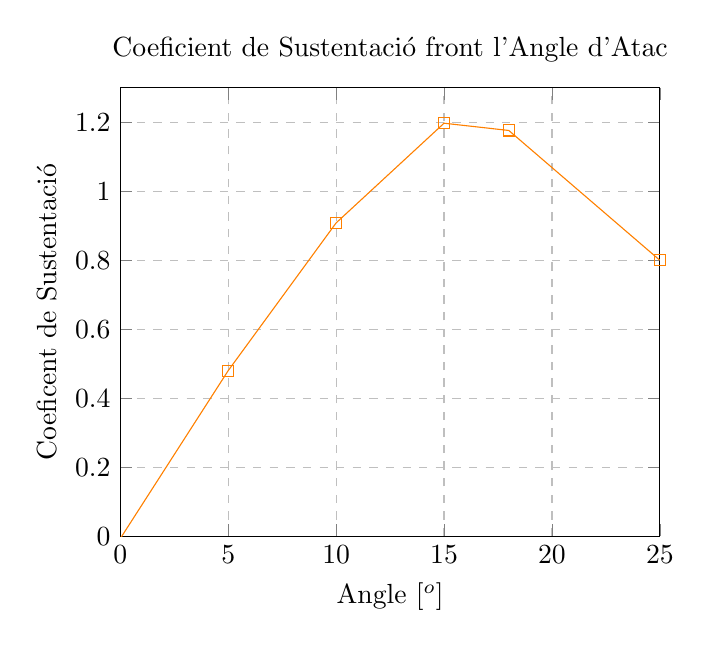
\begin{tikzpicture}
      \begin{axis}[
          title={Coeficient de Sustentació front l'Angle d'Atac},
          xlabel={Angle [$^o$]},
          ylabel={Coeficent de Sustentació},
          xmin=0, xmax=25,
          ymin=0, ymax=1.3,
          xtick={0,5,10,15,20,25},
          ytick={-0.1,0,0.2,0.4,0.6,0.8,1,1.2},
          ymajorgrids=true,
          xmajorgrids=true,
          grid style=dashed,
          ]
      \addplot[
        color=orange,
        mark=square,
        ]
        coordinates {
        (0,-0.007)(5,0.48)(10,0.9084)(15,1.1975)(18,1.1765)(25,0.8)
        };
      \end{axis}
    \end{tikzpicture}
  \end{frame}

% SLIDE : ______________________________________________________________________
  \begin{frame}{Frame Name}
    \centering
    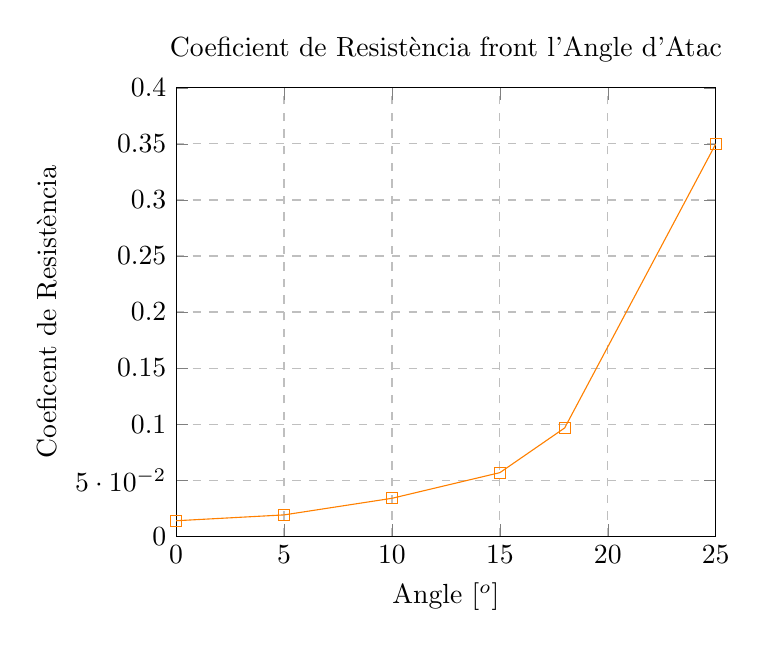
\begin{tikzpicture}
      \begin{axis}[
          title={Coeficient de Resistència front l'Angle d'Atac},
          xlabel={Angle [$^o$]},
          ylabel={Coeficent de Resistència},
          xmin=0, xmax=25,
          ymin=0, ymax=0.4,
          xtick={0,5,10,15,20,25},
          ytick={0,0.05,0.1,0.15,0.2,0.25,0.3,0.35,0.4},
          ymajorgrids=true,
          xmajorgrids=true,
          grid style=dashed,
          ]
      \addplot[
        color=orange,
        mark=square,
        ]
        coordinates {
        (0,0.013779)(5,0.019)(10,0.033807)(15,0.05671)(18,0.09658)(25,0.35)
        };
      \end{axis}
    \end{tikzpicture}
  \end{frame}

% ENDING: ======================================================================

\maketitle

\end{document}
